% ============================================================
% Chapter 4: Equation Database and Test Case Construction — 本文（Phase 2, 2026-08-09）
% 骨子版（Phase 1）は git 履歴の commit bf41ec4 以前を参照。
% 用語の改訂（2026-08-09）: 旧「original / multi-source / DAE」を as-published / cross-document /
%   synthesized に改称した。
% 訂正（2026-09-28）: as-published の定義「文献が 1 つのモデルとして掲載する式集合」は生成コードと
%   矛盾していた。実際は Gemini 2.5 Pro が式 ID・出典・分野名・変数記号だけのカタログから「必要十分かつ
%   最小」の組を選び、のちに自由度検査で解けないものを除いた（generate_training_cases.py,
%   filter_solvable_cases.py）。また LLM 生成の基礎式集（handbook_*）は文献でないため、族名・列名・本文の
%   document を source に改めた: as-published → single-source, cross-document → cross-source,
%   Documents spanned → Sources spanned。cross-source の「共有変数でつなぐ」も 189 件で成り立たないので訂正。
% 数値はすべて一次データ（unified_equations.json, training_cases.json）から実測。
% ============================================================
\section{Equation Database Construction}

We built an equation database of 11,146 equations drawn from 361 sources.
% source: unified_equations.json 実測（式 11,146、source_id 361 種）
Of these sources, 329 are documents and contribute 10,476 equations. A large language model
(Gemini 2.5 Pro\cite{Gemini25}) read each document and returned every equation in the text
together with its symbols, the sentences around it, and a domain label. The remaining 32 sources
are reference equation sets that the same model generated domain by domain to cover textbook
fundamentals; these 670 equations have no source document.
% source: unified_equations.json 実測（handbook_* 以外 329 種 = 10,476 式：.pdf 328 種 10,437 式
%         ＋技術報告 ORNL/SPR-2018/864 の 39 式。handbook_* 32 種 = 670 式、Gemini 2.5 Pro が生成：
%         handbook_chemeng は build_equation_graph.py、他 31 種は expand_dataset.py）;
%         processed_pdfs.json は 339 件処理済み。2026-09-28 訂正: 旧記載「PDF 328 種・基礎式集 33 種
%         709 式」は ORNL 報告を基礎式集に数えていた
Each database entry holds the \LaTeX{} expression of the equation, its variable set, its
surrounding text, its source, and its domain label. The database grew from 3,244 to 11,146
equations during this work, and the added documents span engineering fields beyond chemical
engineering.

Two properties of the database govern the difficulty of retrieval, and we state them here because
every later result depends on them. First, we match variables across sources by their raw symbols
and apply no notational normalization, so the database holds 13,220 distinct variable symbols and
treats notational variants of one quantity, such as $C_A$ and $C_A(t)$, as different variables.
% source: unified_equations.json 実測（eq_vars の和集合 13,220 種）; two_stage_query_conditioned.py
%         norm() は strip() のみ（記号の正規化なし）
Retrieval across documents is therefore harder than a shared notation would make it, and the
variable-overlap features of Chapter~3 read a conservative signal. Second, the domain labels are
free text written by the extractor rather than entries of a fixed taxonomy: the 11,146 equations
carry 1,998 distinct labels, 27.9\% of which occur exactly once, and a single source carries 6.36
labels on average.
% source: unified_equations.json 実測（1,998 ラベル、singleton 27.9\%、source あたり 6.36 種）
Exact agreement between two labels is consequently rare, which Section~\ref{sec:nullresult} shows to be one reason
the domain features contribute nothing.

\section{Test Cases}

Each test case pairs a query --- a description with its input and output variables --- with the
ground-truth equation set that composes the requested model. We built 2,838 cases in three
evaluation families and one training-only family, and Table~\ref{tab:families} summarizes them.
% source: training_cases.json variant_type 集計（original 92; multisource_* 731;
%         dae_X1..X10 各100 = 1,000; random_io_from_models 738 + context_paraphrased 276 + swap_io 1
%         = 1,015）。K・文献数は correct_model_ids から実測。

We name the families by where their equations come from and how their ground truth was formed.
A language model chose the ground truth of the single-source family. We gave Gemini 2.5 Pro a
catalog that listed, for each database equation, only its identifier, source, domain label, and
variable symbols --- neither the equation nor its surrounding text --- and asked for cases whose
equations determine the outputs from the inputs and are ``sufficient and minimal.'' A
degree-of-freedom check then kept only the cases whose equations, once the inputs are given, have
exactly as many unknowns as equations. The ground truth is therefore the set that the language
model judged minimal, not the model that a source presents: 67 of the 92 cases need a single
equation, and 61 draw on the generated reference sets rather than on documents.
% source: generate_training_cases.py（カタログは model_id・source_id・eq_id・domain・variable_symbols
%         のみ、プロンプト "sufficient and minimal (no redundant equations)"、gemini-2.5-pro）;
%         filter_solvable_cases.py（|unknown| == 式数）; training_cases.json 実測（K=1 が 67 件、
%         正解式がすべて handbook_* の件が 61 件）。例: core_020_v1 は Marlin の教科書が 5 式
%         (14.1)-(14.5) で「DOF = 5 - 5 = 0」と書く系から (14.4) の 1 式だけを正解にしている
The cross-source family combines equations of two or three sources. An algorithm formed 500 of its
cases by pairing equations that share at least two variables; the other 231 are input--output
variants of 33 combinations that an LLM coding assistant wrote and a degree-of-freedom check
verified, and in 189 of them the equations share no variable. The synthesized family grows each
ground truth by rule to a prescribed size (Section~4.3).
% source: generate_multisource_v3.py（multisource_v3 500 件、共有変数 2 個以上: 実測 2 個 398・3 個 92・
%         4 個以上 10）; generate_multisource_cases.py（multisource_original 33 件、docstring「Claude が
%         手作業で作成し自由度ゼロを機械的に検証」）＋ expand_multisource_variants.py（random_io 198 件）;
%         変数記号の共有なし 189 件（original 27 + random_io 162）は実測

\begin{table}[H]
\centering
\caption{The four case families. ``Equations per case'' gives the mean and maximum size of the
ground-truth set, and ``sources spanned'' the mean number of sources it draws on, where a
generated reference set counts as one source. The released data identifies the families as
\texttt{original}, \texttt{multisource\_*}, \texttt{dae\_X1}--\texttt{dae\_X10}, and the
augmentation variants respectively.}
\label{tab:families}
\small
\begin{tabular}{llccl}
\toprule
Family & How the ground truth was defined & \begin{tabular}[c]{@{}c@{}}Cases\end{tabular} &
\begin{tabular}[c]{@{}c@{}}Equations\\per case\end{tabular} &
\begin{tabular}[c]{@{}l@{}}Sources\\spanned\end{tabular} \\
\midrule
Single-source  & A language model picks, from one source, a set & 92 & 1.34 (4) & 1.01 \\
               & \quad it judges sufficient and minimal & & & \\
Cross-source   & We combine equations of two or three sources & 731 & 2.03 (3) & 2.02 \\
Synthesized    & We grow a closed system to a prescribed size $X$ & 1{,}000 & 5.50 (10) & 1.10 \\
\midrule
Augmented      & We perturb the I/O variables or paraphrase the & 1{,}015 & 1.57 (4) & 1.02 \\
(training only)& \quad description of a case above & & & \\
\bottomrule
\end{tabular}
\end{table}

The families differ in provenance as well as in size. Every cross-source case spans at least two
sources by construction, and none spans more than three; the single-source and synthesized
families stay within one source in 98.9\% and 95.9\% of their cases.
% source: 実測（source_id 単位。cross-source は 100\% が 2 出典以上・最大 3、single-source 1.1\%
%         （1 件）、synthesized 4.1\% が 2 出典以上・最大 9）
The synthesized family is also by far the largest in answer size, and it carries the evaluation of
set selection: 90.8\% of the 1,823 evaluation cases need two or more equations, and they need 3.90
on average.
% source: 実測（設定A 1,823件: K>=2 が 90.8\%、平均 K = 3.90。全 2,838 件では K>=2 が 74.6\%）
We exclude the augmented family from every evaluation, because perturbed copies of a case inflate
the baseline and hide the difficulty that motivates the method (Section~5.1).

Two properties of the construction limit what the experiments can claim, and we record them here.
First, in the cross-source and synthesized families the number of ground-truth equations equals
the number of output variables in every case, and in the single-source family it does so in
92.4\% of the cases.
% source: 実測（K == |O| の割合: single-source 92.4\%、cross-source 100\%、synthesized 100\%）
Predicting the answer size from the query is therefore close to trivial in this dataset, so
Section~\ref{sec:dofstopresults} evaluates DoF-stop on closure and set quality rather than on size prediction.
Second, every case takes its input and output variables from the symbols of its ground-truth
equations, so a query and its answer share one notation by construction.
% source: 実測（入出力変数 ⊆ 正解式の変数記号の和集合: 4 族とも 100\%）;
%         generate_training_cases.py の "input/output variables MUST be subsets of variable_symbols"

\section{Synthesized Case Generation}

Our earlier cases were biased toward small and purely algebraic systems, so we regenerated the hard
part of the dataset as differential--algebraic systems that are solvable by construction. The
procedure, proposed by Mr.~Kato, starts from an ordinary differential equation and takes its
differentiated variable as an output. It then repeatedly adds an equation that shares a non-output
variable with the current set, and it stops at the target size $X$. We accept only square systems,
in which the number of unknowns equals the number of equations, and each equation contributes an
output variable of its own, so every unknown can be matched to its own equation.
% source: generate_dae_cases.py L302-330（追加式ごとに、その式の変数から出力を 1 つ選ぶ。入力＝残りの変数）;
%         実測（2026-09-29）: 合成 1,000 件すべてで式と未知変数の完全マッチングが存在（Hopcroft--Karp）
% source: docs/progress_report_2026-06-14_seminar.tex §5（手順ボックス）; 実装 generate_dae_cases.py
We generated 100 cases for each $X = 1, \dots, 10$, giving 1,000 cases. A large language model
(Anthropic Claude) writes only the natural-language description; the equation set, the input
variables, and the output variables all follow from the rule-based procedure.

A continuous stirred-tank reactor gives the smallest interesting example: the mass-balance ordinary
differential equation, the reaction-rate equation $r_A = k C_A$, and the Arrhenius equation
$k = A \exp(-E / RT)$ form a closed system of three equations. Appendix~A shows one generated case
in full. Because the construction guarantees that a solvable answer exists, a failure to retrieve
it is a failure of the method rather than of the dataset.

\section{Stratified Source-disjoint Splitting}

We assign each source wholly to training, validation, or testing, in roughly a $6{:}2{:}2$
ratio. A random split of cases would leak answers, because a paraphrased copy of a case could land
in training while the case itself lands in testing, and both share the same ground-truth equations.
% source: docs/progress_report_2026-06-14_seminar.tex §4; 実装 set_aware_reranker.py
%         stratified_src_split
Source-disjoint assignment removes that leak, but it introduces a new problem: a random assignment
of sources can put the hard cases on one side and make the score depend on the draw rather than on
the method.

We therefore stratify the assignment. Among 400 random candidate assignments we select the one that
minimizes the summed $L_1$ distance between the training and test distributions of four
difficulty-related quantities: the number of equations, the number of input variables, the number of
output variables, and the number of sources spanned. Every experiment repeats over the same 10
random seeds and reports the mean and the spread across them. Results therefore measure
generalization to unseen sources rather than memorization of seen ones.

\begin{figure}[H]\centering
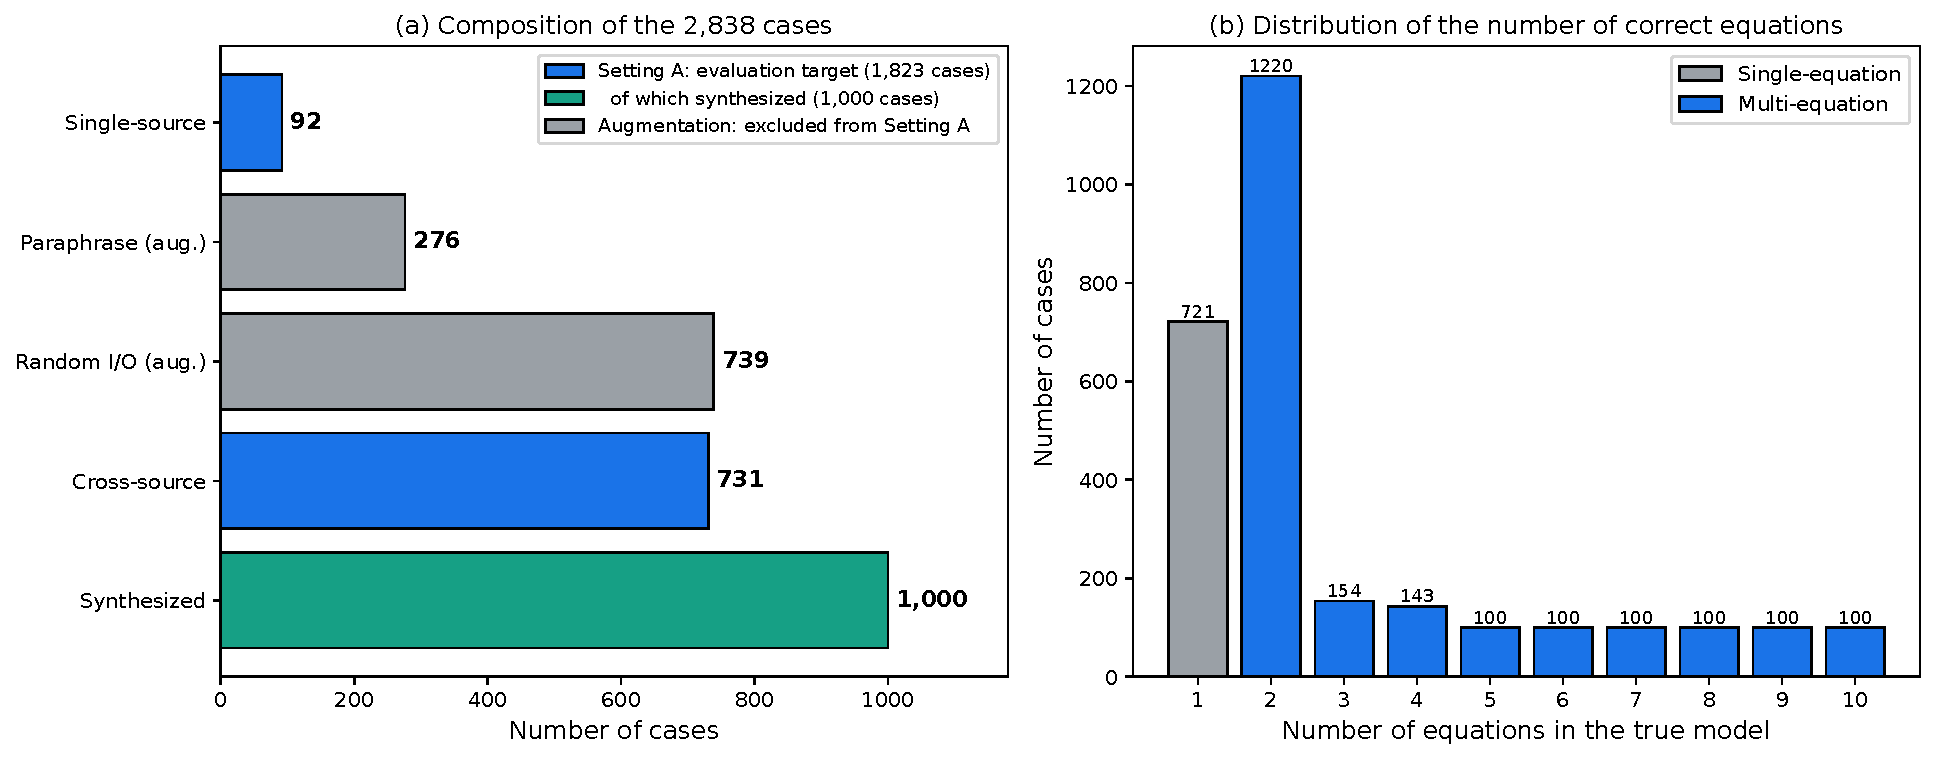
\includegraphics[width=0.6\linewidth]{figures/fig_dataset.pdf}
\caption{Composition of the 2,838 cases and the distribution of the number of ground-truth
equations. The evaluation set (1,823 cases) excludes the augmented family.}
\label{fig:dataset}
\end{figure}

% 骨子段階は非表示（本文化時に comment 環境を外す）
\begin{comment}
\begin{figure}[H]\centering
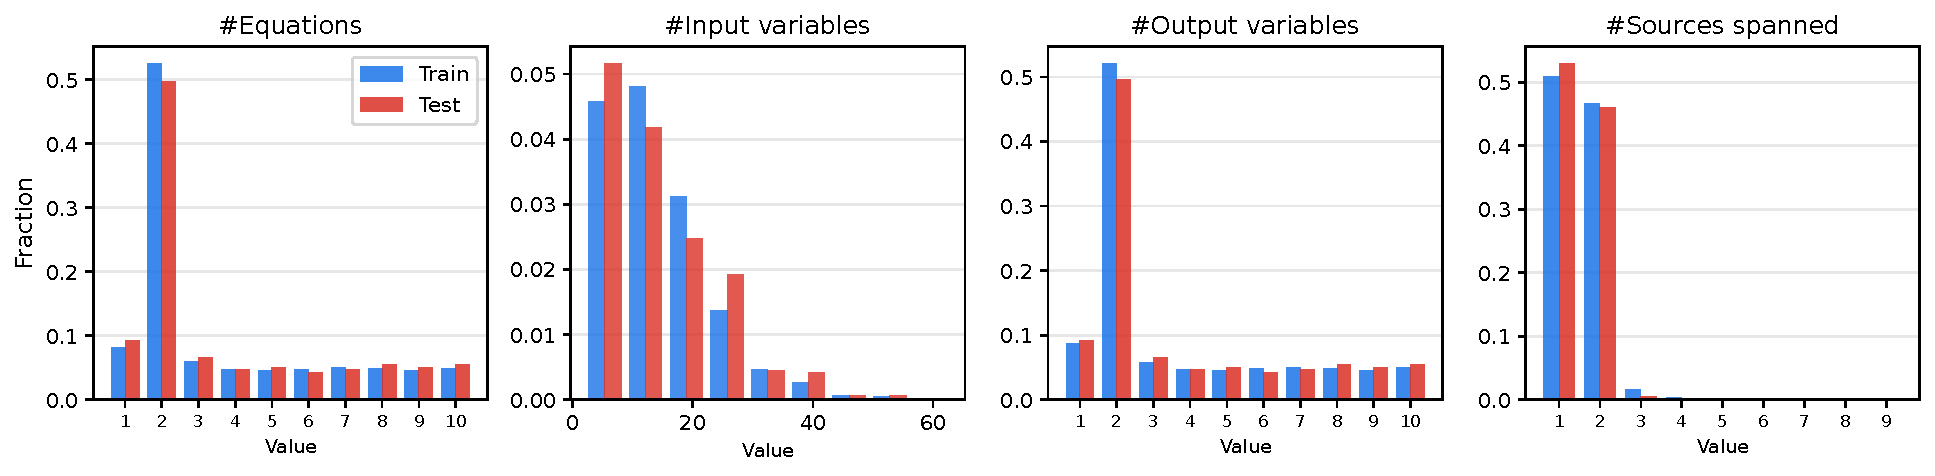
\includegraphics[width=0.6\linewidth]{figures/fig_split_balance.pdf}
\caption{Stratified source-disjoint split: four difficulty-related distributions match between train
(blue) and test (orange); one seed shown.}
\label{fig:split}
\end{figure}
\end{comment}
